%%%%%%%%%%%%%%%%%%%%%%%%%%%%%%%%%%%%%%%%%%%%%%%%%%%%%%%%%%%%%%%%%%%%%
%
% VC36O Writeup Template
%
% This is a LaTeX document. LaTeX is a markup language for producing 
% documents. Your task is to fill out this
% document, then to compile this into a PDF document. 
% You will then upload this PDF to `Moodle'.
%
% 
% TO COMPILE:
% > pdflatex thisfile.tex
%
% For references to appear correctly instead of as '??', you must run 
% pdflatex twice.
%
% If you do not have LaTeX and need a LaTeX distribution:
% - Personal laptops (all common OS): www.latex-project.org/get/
%
% If you need help with LaTeX, please come to office hours. 
% Or, there is plenty of help online:
% https://en.wikibooks.org/wiki/LaTeX
%
% Good luck!
%
%%%%%%%%%%%%%%%%%%%%%%%%%%%%%%%%%%%%%%%%%%%%%%%%%%%%%%%%%%%%%%%%%%%%%
%
% How to include two graphics on the same line:
% 
% \includegraphics[\width=0.49\linewidth]{yourgraphic1.png}
% \includegraphics[\width=0.49\linewidth]{yourgraphic2.png}
%
% How to include equations:
%
% \begin{equation}
% y = mx+c
% \end{equation}
% 
%%%%%%%%%%%%%%%%%%%%%%%%%%%%%%%%%%%%%%%%%%%%%%%%%%%%%%%%%%%%%%%%%%%%%%%%%%%%%%%%%%%%%%%%%%%%%%%%

\documentclass[11pt]{article}

\usepackage[english]{babel}
\usepackage[utf8]{inputenc}
\usepackage[colorlinks = true,
            linkcolor = blue,
            urlcolor  = blue]{hyperref}
\usepackage[a4paper,margin=1.5in]{geometry}
\usepackage{stackengine,graphicx}
\usepackage{fancyhdr}
\setlength{\headheight}{15pt}
\usepackage{microtype}
\usepackage{times}
\usepackage{booktabs}

% From https://ctan.org/pkg/matlab-prettifier
\usepackage[numbered,framed]{matlab-prettifier}

\frenchspacing
\setlength{\parindent}{0cm} % Default is 15pt.
\setlength{\parskip}{0.3cm plus1mm minus1mm}

\pagestyle{fancy}
\fancyhf{}
\lhead{Project Writeup}
\rhead{VC36O 2018/1}
\rfoot{\thepage}

\date{}

\title{\vspace{-1cm}Project 2 Writeup}


\begin{document}
\maketitle
\vspace{-3cm}
\thispagestyle{fancy}

\section*{In the beginning...}
Em processamento de imagens, trabalha-se com tons de cinza, conhecidos como \textit{digital number} ou DNs, que são atribuídos aos pixeis de uma imagem. O histograma é uma das formas mais comuns de se representar a distribuição DNs de uma imagem. Ele fornece a informação sobre quantos pixeis na imagem possuem cada valor possível de DN (no caso das imagens de 8 bits, variam de 0 a 255) ou, de forma equivalente, onde a proporção da imagem que corresponde a cada valor de DN \cite{hist}.

Os histogramas também são conhecidos como distribuição de intensidades ou Função de Densidade de Probabilidade (PDF). Esse último termo deriva do fato de que, estatisticamente, o histograma representa, a probabilidade de se achar um DN de um dado valor dentro de uma imagem \cite{hist}.

Ao se observar o histograma de uma imagem, tem-se uma noção sobre as características da mesma. A forma do histograma fornece informações de grande importância da imagem, tal como intensidade média e espalhamento dos valores de DN; este último, por sua vez, dá a medida do contraste de uma imagem: quanto maior o espalhamento ao longo do eixo dos DNs, maior o contraste da imagem (Figura~\ref{fig:hist}) \cite{hist}.

\begin{figure}[h]
    \centering
    \includegraphics[width=8cm]{imagem28.JPG}
    \caption{Histograma de uma imagem separados por canais RGB.}
    \label{fig:hist}
\end{figure}

Em processamento de imagens, existe uma técnica denominada correspondência ou especificação de histograma que é a transformação de uma imagem para que seu histograma corresponda a um histograma especificado \cite{wiki}. 

Um detector pode ser usado para normalizar duas imagens, quando as essas foram adquiridas na mesma iluminação local (como sombras) sobre o mesmo local, mas por diferentes sensores, condições atmosféricas ou iluminação global \cite{wiki}.

Imagens com valores de pixeis de 8 bits, a correspondência de histogramas só pode aproximar o histograma especificado. Todos os pixeis de um determinado valor na imagem original devem ser transformados em apenas um valor na imagem de saída \cite{wiki}.

Existem diversas técnicas propostas para resolver o problema de correspondência de histograma, uma delas é por meio do Recozimento simulado - \textit{Simulated Annealing}.


O Recozimento simulado é uma meta-heurística para otimização que consiste numa técnica de busca local probabilística, e se fundamenta numa analogia entre o modo como um metal se resfria e congela numa estrutura cristalina de energia mínima e a busca por um mínimo num sistema qualquer \cite{simulated}. 

A cada iteração, o algoritmo do Recozimento simulado, procura o próximo candidato a ponto de mínimo na vizinhança do candidato corrente, agindo de acordo com a diferença entre os valores da função-objetivo (função de energia ou potencial). A maior vantagem desse algoritmo é a possibilidade de evitar mínimos locais, para isso, é realizada uma busca aleatória que, por vezes, aceita vizinhos cuja energia seja mais elevada. Ou seja, em algumas iterações, o Recozimento simulado tende a maximizar a função-objetivo em vez de minimizá-la. Entretanto a probabilidade de se aceitar um vizinho de maior energia cai com o tempo \cite{simulated}.


Para realizar a correspondência de histograma de uma imagem por meio da solução do Recozimento simulado, foi utilizado a linguagem Octave. As imagens utilizadas foram tiradas de um mesmo local, porém a que foi modificada seu histograma possui variação na sua intensidade, ou seja, ela está mais avermelhada (Figura~\ref{fig:imagens}).

\begin{figure}[h]
    \centering
    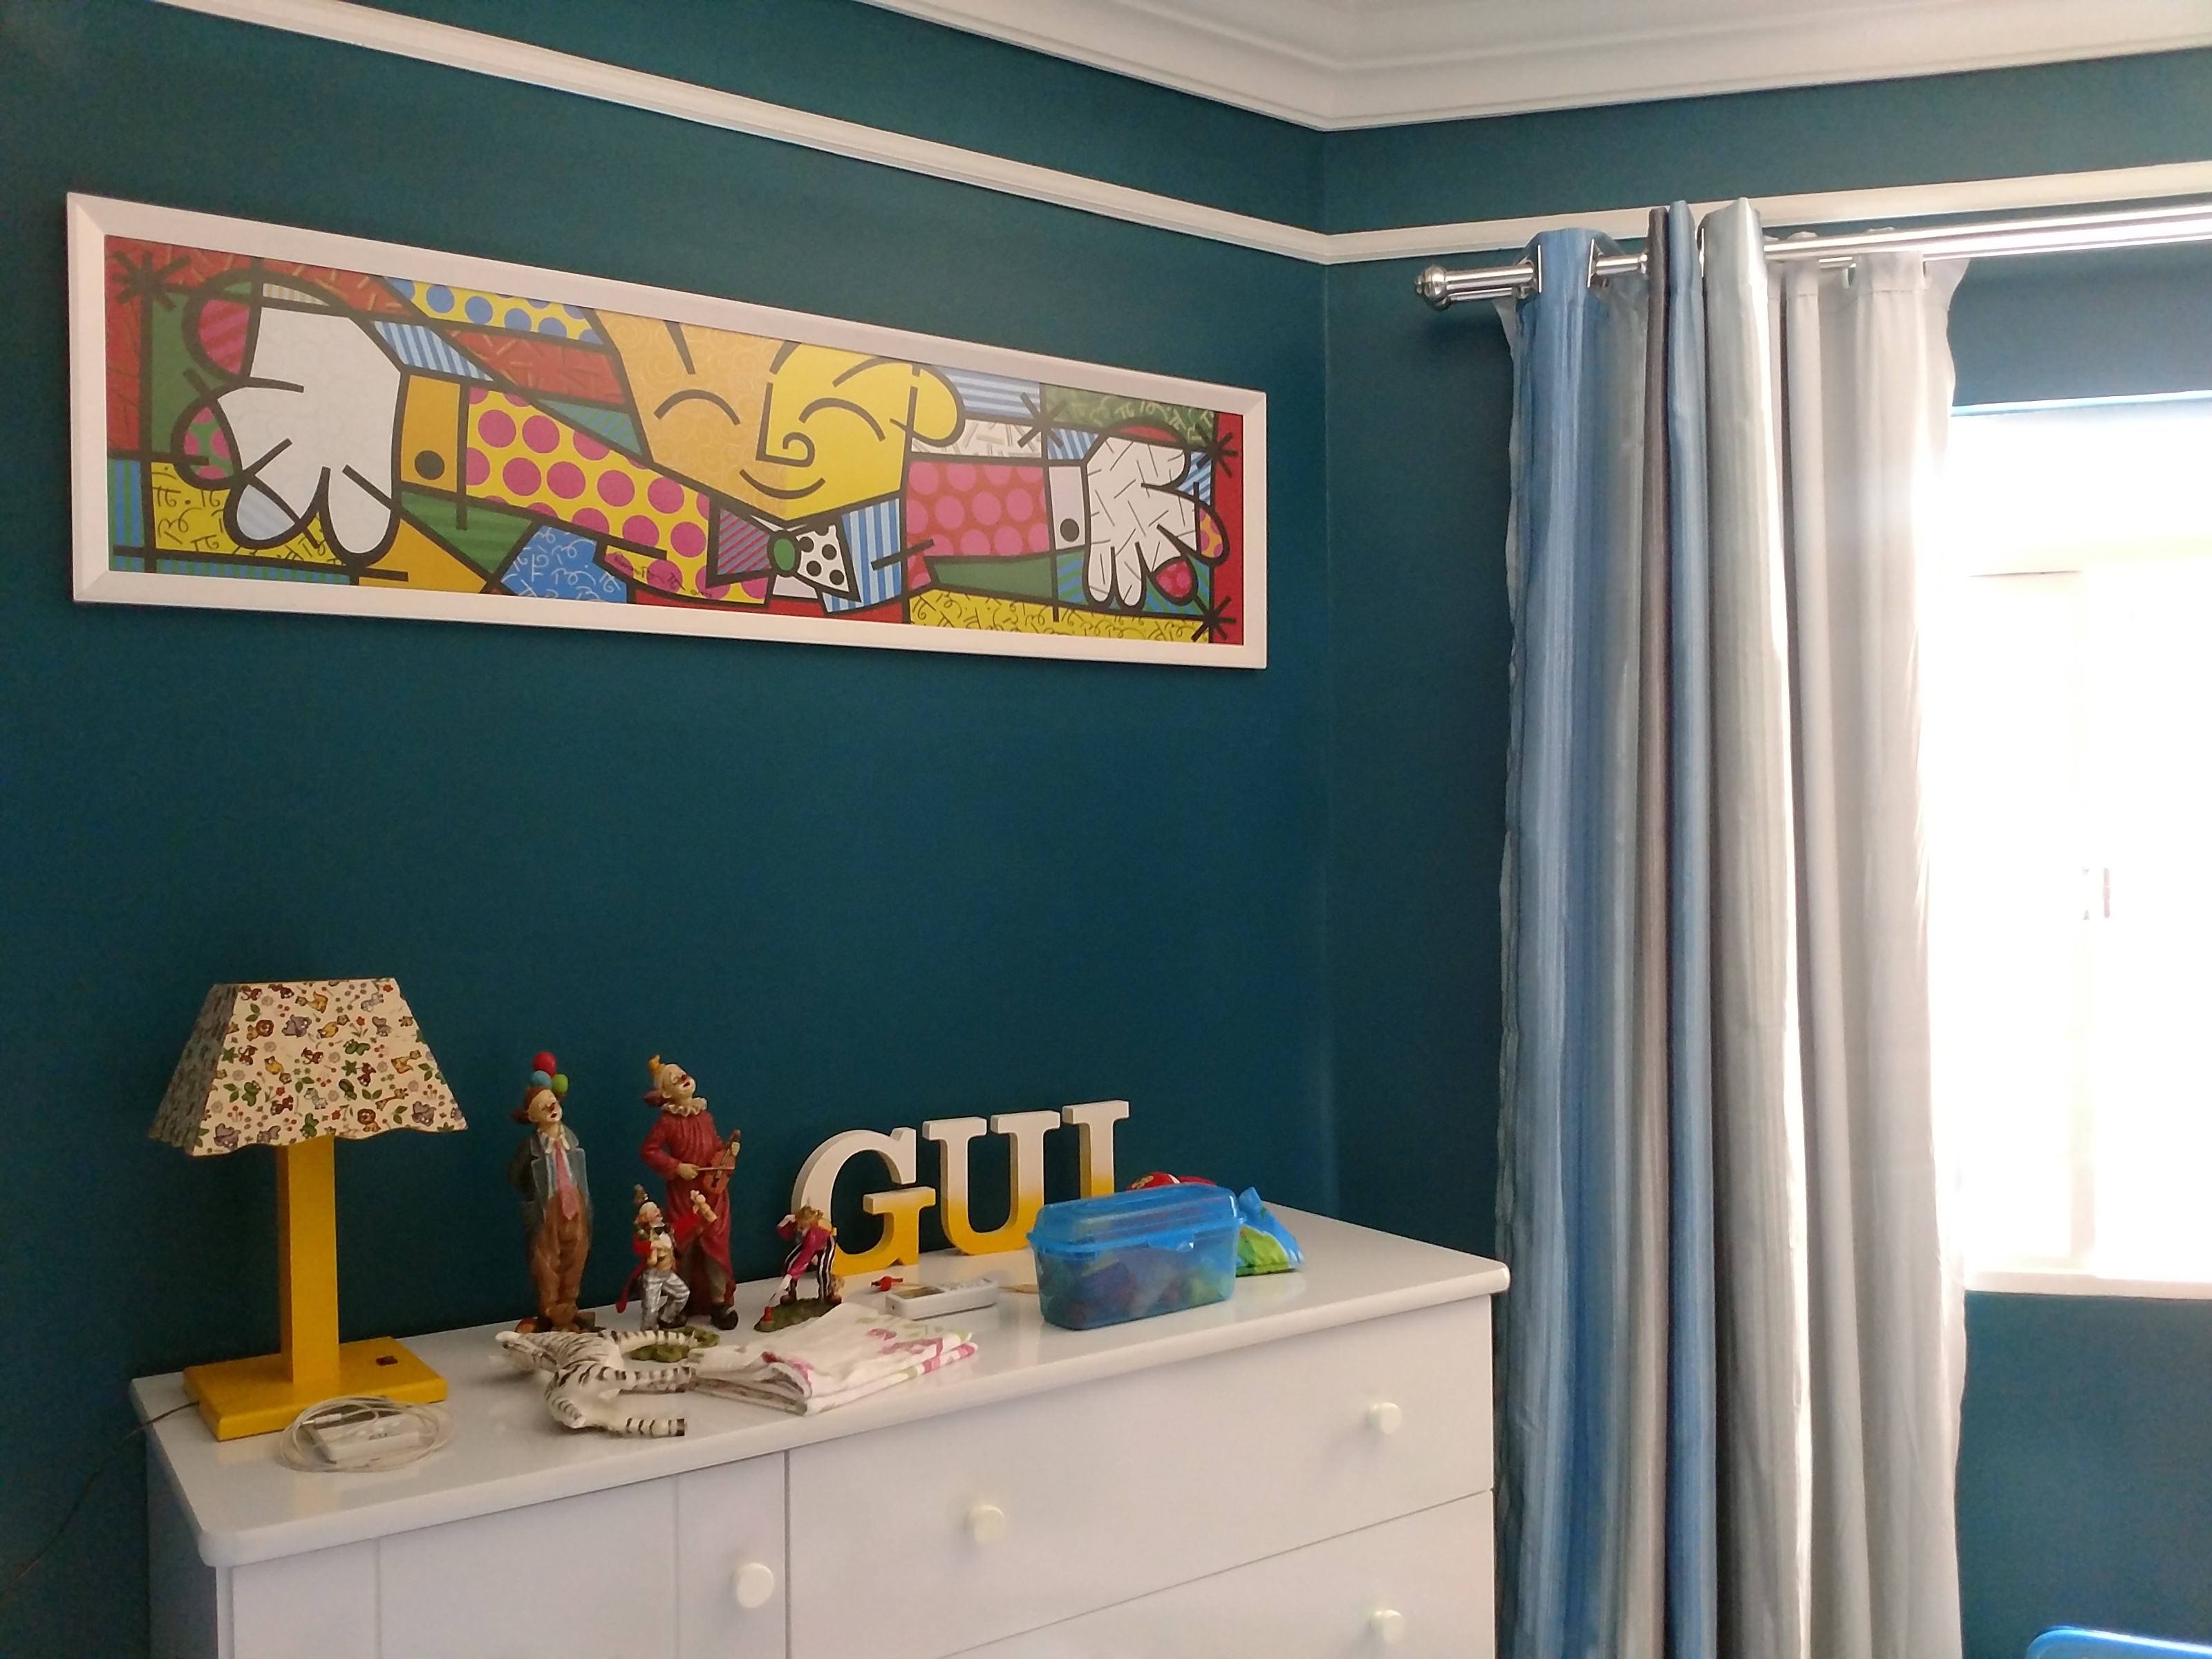
\includegraphics[width=5cm]{../data/img1.jpg}
    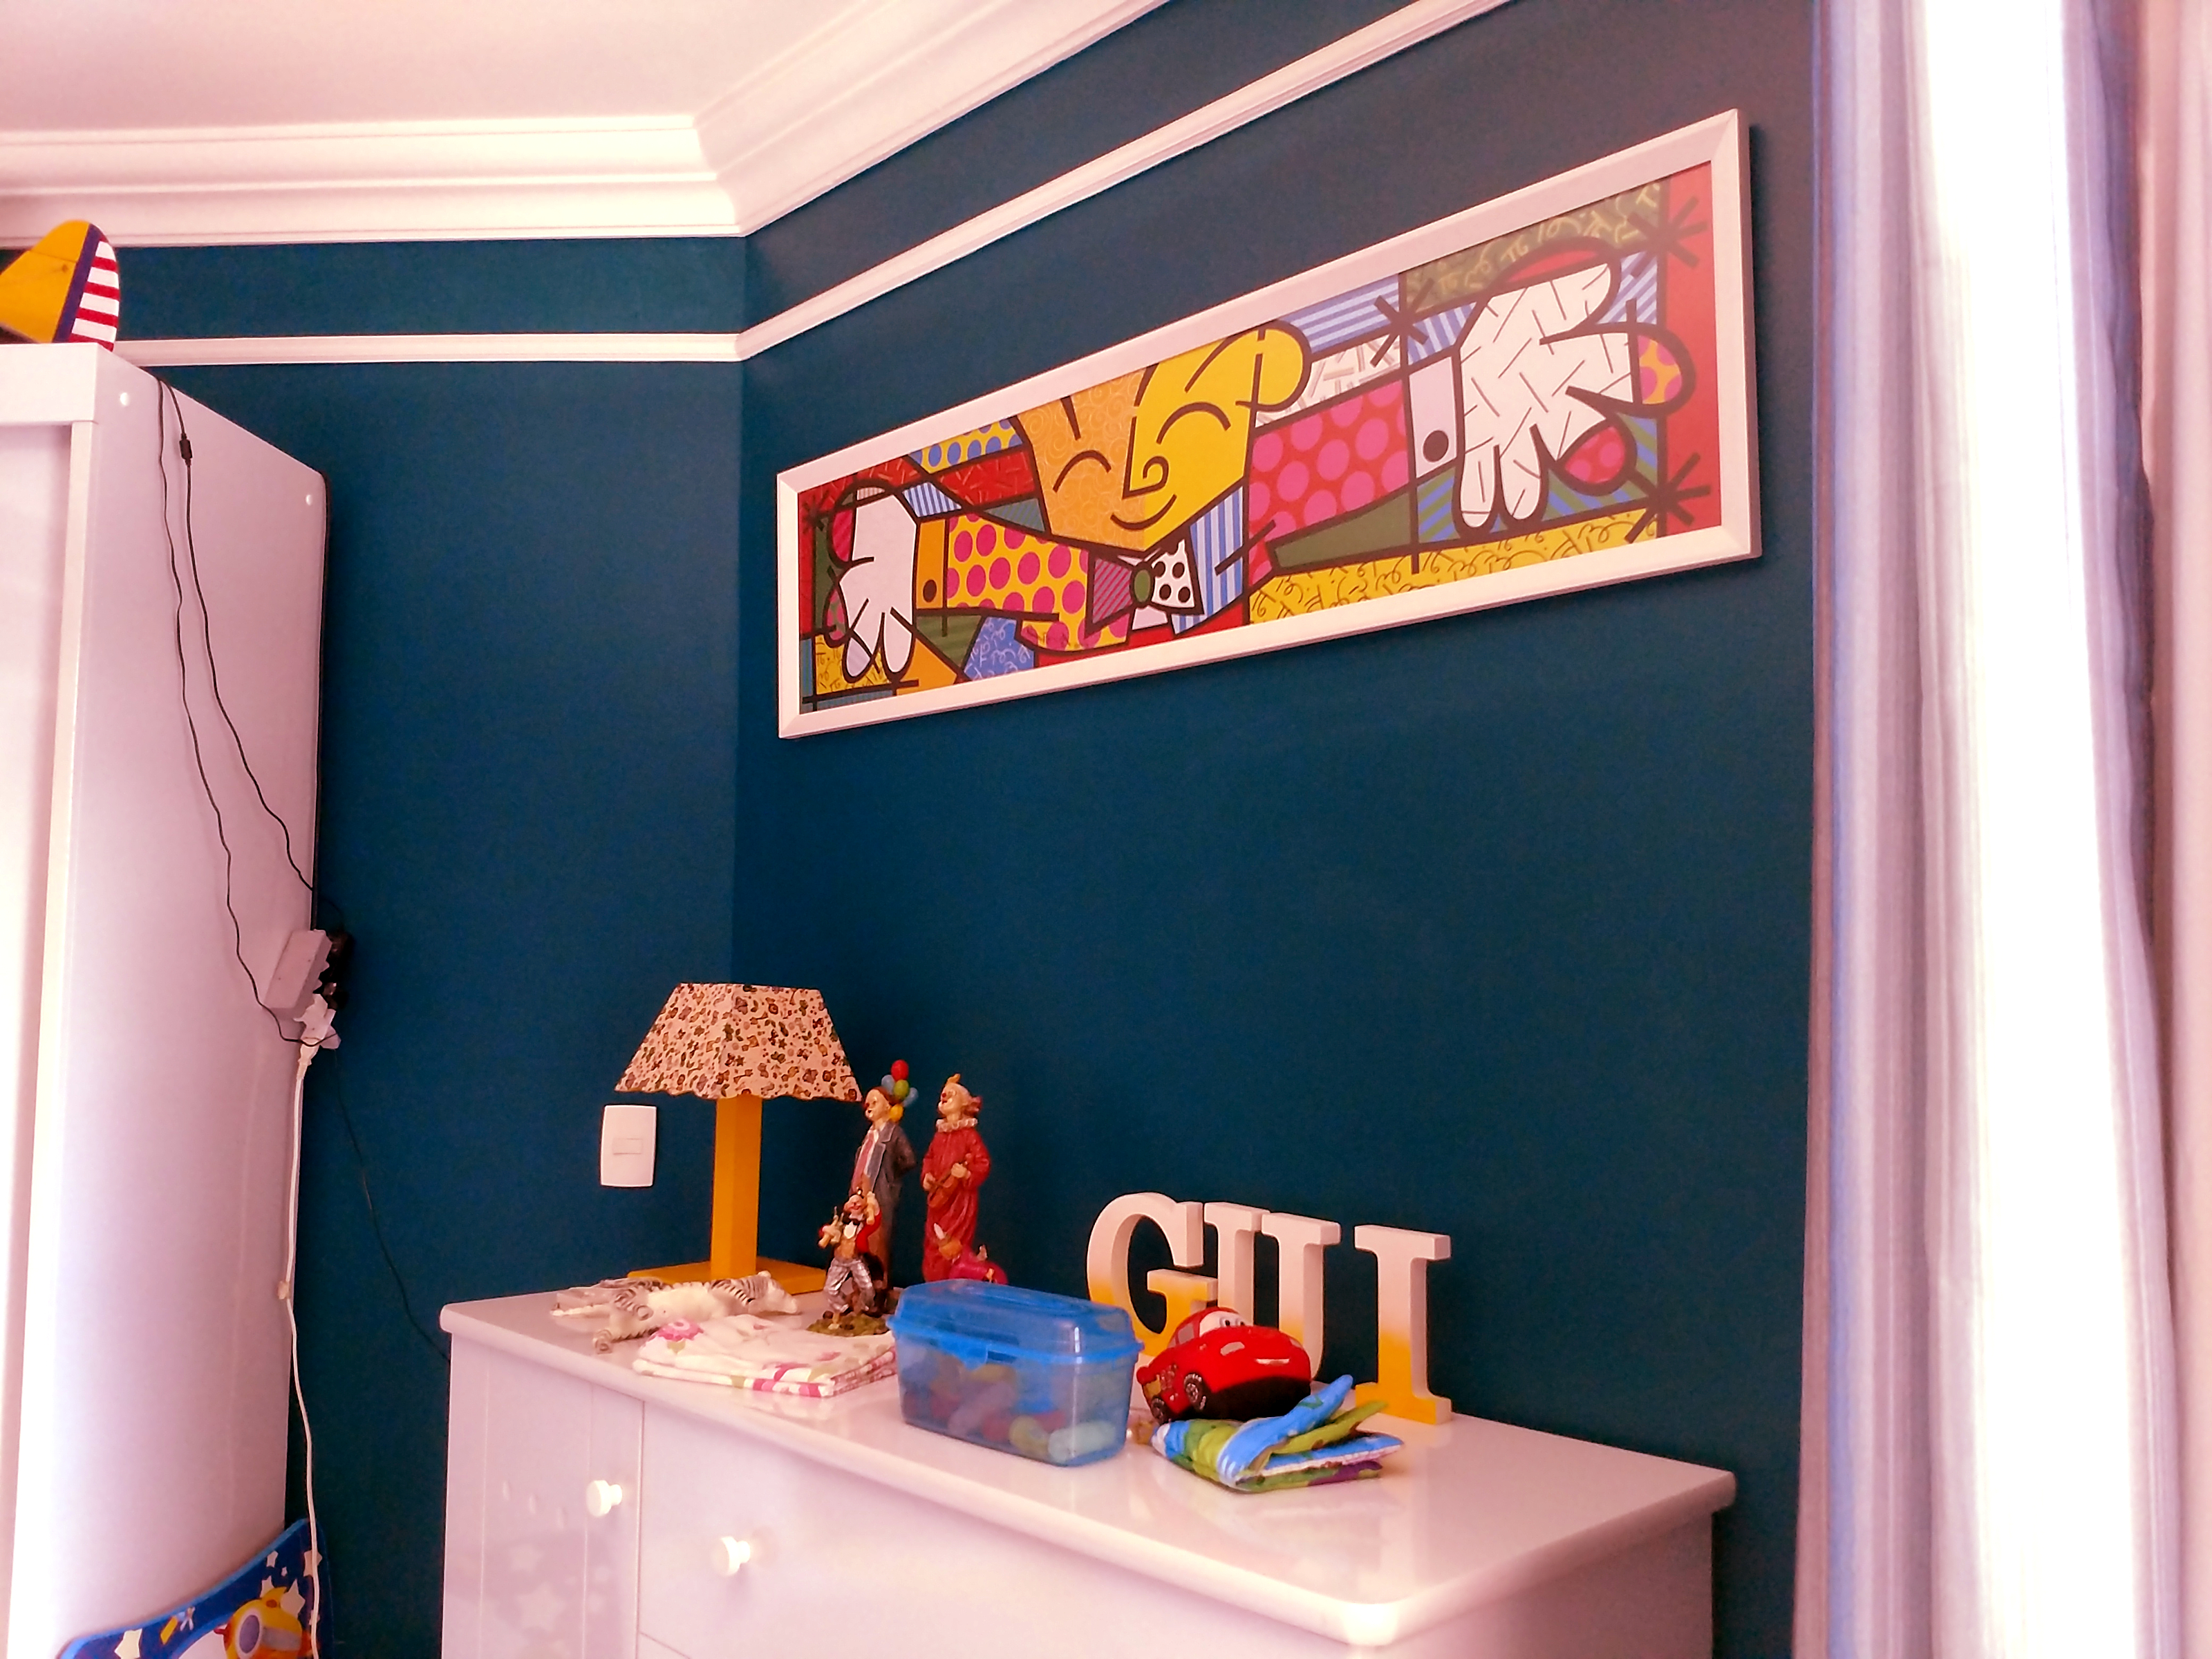
\includegraphics[width=5cm]{../data/img2.jpg}
    \caption{\emph{Esquerda:} Imagem original. \emph{Direita:} Imagem modificada.}
    \label{fig:imagens}
\end{figure}

Inicialmente, as imagens trabalhadas foram partes da imagem original (Figura~\ref{fig:imagensPatch}), pois dessa forma acelerou o mapeamento do Recozimento simulado, e solução obtida pelo algorismo foi aplicada a imagem modificada de tamanho original (\ref{fig:imagens}). 

\begin{figure}[h]
    \centering
    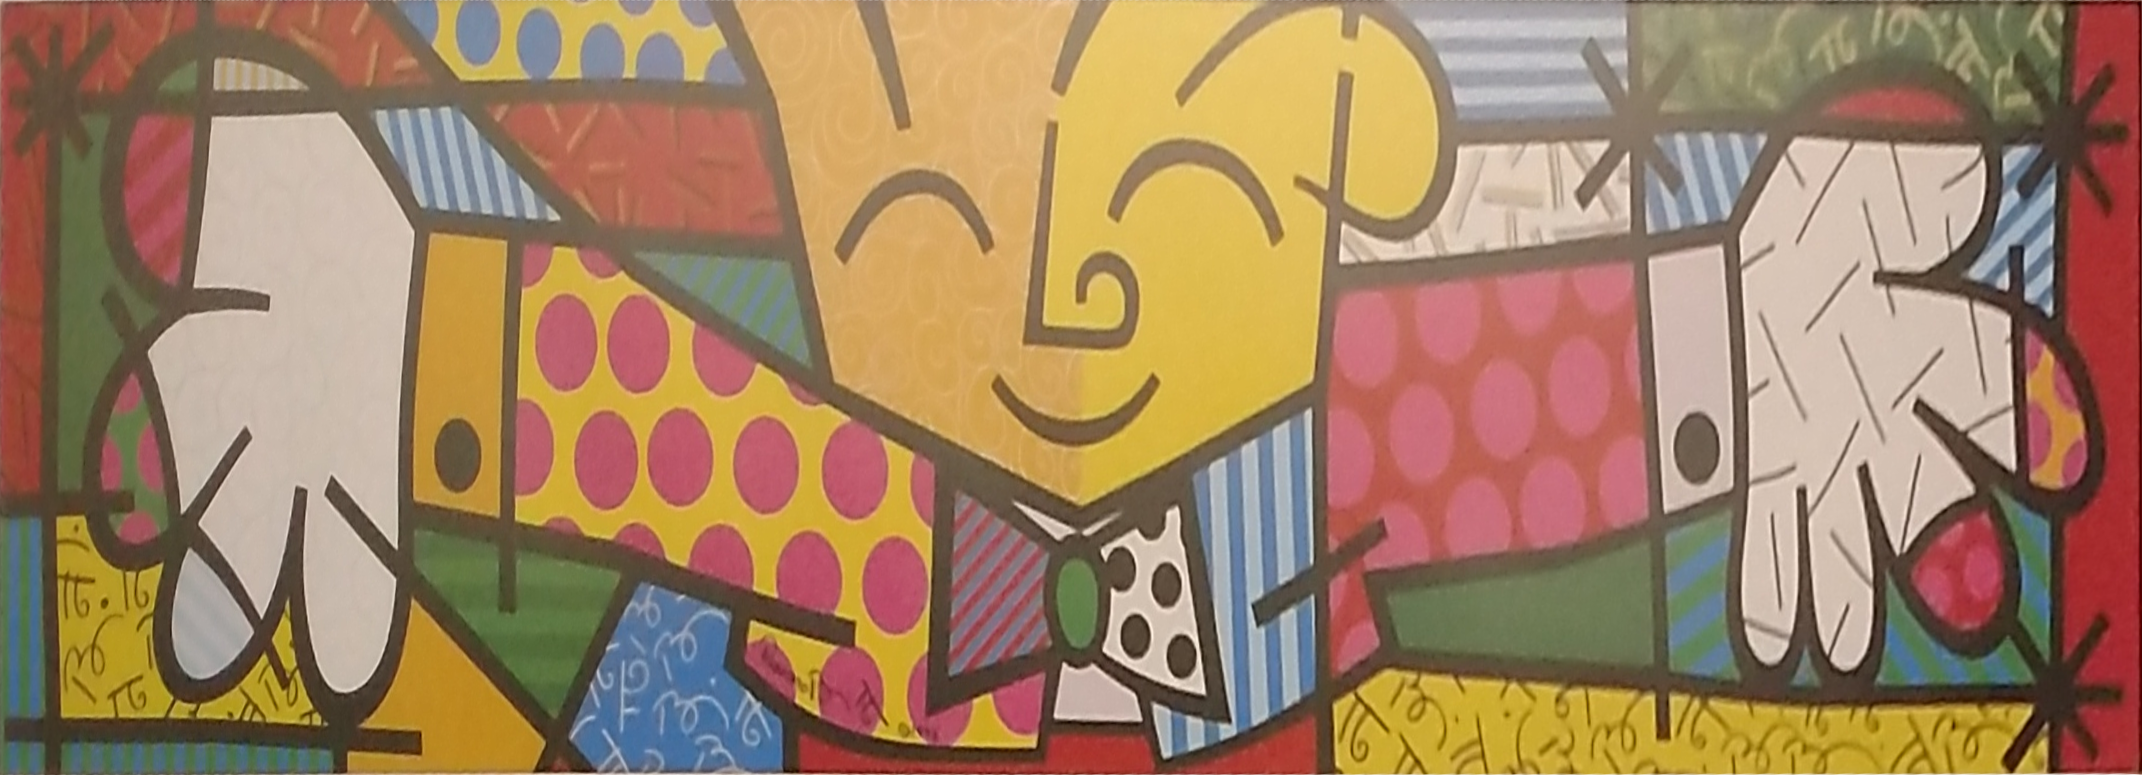
\includegraphics[width=5cm]{../data/img1_patch.jpg}
    \includegraphics[width=5cm]{../data/img2_patch.jpg}
    \caption{\emph{Esquerda:} Patch da imagem original. \emph{Direita:} Patch da imagem modificada.}
    \label{fig:imagensPatch}
\end{figure}

O objetivo do código foi mapear: o histograma do patch da imagem modificada de forma que se aproximasse do histograma do patch da imagem original, e o histograma da imagem modificada  para se aproximar do histograma da imagem original.

Para atingir o objetivo, os canais RGB das imagens modificadas foram separados e trabalhados individualmente, ou seja, foram mapeado os histogramas dos canais vermelho, verde e azul, depois esses foram juntados novamente para formar a imagem colorida final modificada. Cada canal retorna uma imagem em escala cinza, com intensidades de 0 a 255.



\section*{Interesting Implementation Detail}
Inicialmente, o código deve carregar as imagens e separar seus canais RGB. Isso é feito em arquivo chamado \texttt{Proj2.m}, que está descrito abaixo:

\begin{lstlisting}[style=Matlab-editor]
image1 = imread('../data/img1.jpg');
image2 = imread('../data/img2.jpg');
image1patch = imread('../data/img1_patch.jpg');
image2patch = imread('../data/img2_patch.jpg');

% Canais RGB PATCH1
red = image1patch(:,:,1); % Canal vermelho
green = image1patch(:,:,2); % Canal verde
blue = image1patch(:,:,3); % Canal azul

% Canais RGB PATCH2
red2 = image2patch(:,:,1); % Canal vermelho
green2 = image2patch(:,:,2); % Canal verde
blue2 = image2patch(:,:,3); % Canal azul

canalRed = SimulatedAnnealing(red, red2);
canalGreen = SimulatedAnnealing(green, green2);
canalBlue = SimulatedAnnealing(blue, blue2);

% Voltar para imagem original
img_patch2 = cat(3, canalRed, canalGreen, canalBlue);

\end{lstlisting}

As imagens são carregadas nas linhas 1 a 4. As linhas 7, 8 e 9 são responsáveis por separar os canais RGB da imagem patch que não será modificada. Já as linhas 12, 13 e 14 separam os canais RGB da imagem patch que será modificado seu histograma. Feito isso, é chamada a função do Recozimento simulado para cada canal do patch (linhas 16, 17 e 18), no qual retorna uma nova imagem. Ao final, todos as novas imagens dos canais devem ser juntadas (linha 21). As separações dos canais também são aplicadas as imagens com tamanhos originais (\texttt{image1 e image2}).

Antes de iniciar o algoritmo do Recozimento simulado, deve ser definido um estado por um conjunto de 4 pontos posicionados sobre uma grade 256×256 que representa um polinômio de grau 3 que passa por cada um dos 4 pontos. Considere o código a seguir:
 
\begin{lstlisting}[style=Matlab-editor]
%encontra 4 ponstos em x e 4 em y
  intervaloX = 84;
  intervaloY = 85;
  pontos = pontos2 = 1;
  
  for i = 1: 4
    pontosX(i) = pontos;
    pontosY(i) = pontos2;
    pontos += intervaloX;
    pontos2 += intervaloY;
  end  
\end{lstlisting}

As ações das linhas 6 a 11 são responsáveis por definir 4 coordenadas, que apresentam uma diferença de 84 para os pontos x e 85 para os y, ou seja, as coordenadas em x serão 1, 85, 169, 153; e em y 1, 86, 171, 256. Essas coordenadas  são aplicadas na equação de grau 3 para obter 4 coeficientes, que são os 4 pontos responsáveis por mapear a nova intensidade da imagem. A seguir é descrita a função \texttt{resolvSistema} que encontra esses coeficientes:

\begin{lstlisting}[style=Matlab-editor]
function [I] = ResolvSistema(pontosX, pontosY)
  x1 = pontosX(1);
  x2 = pontosX(2);
  x3 = pontosY(3);
  x4 = pontosY(4);

  y1 = pontosY(1);
  y2 = pontosY(2);
  y3 = pontosY(3);
  y4 = pontosY(4);
  
  A = [x1^3,x1^2,x1,1; x2^3,x2^2,x2,1; x3^3,x3^2,x3,1; x4^3,x4^2,x4,1];
  B = [y1; y2; y3; y4];
  [I] = A\B;

end
\end{lstlisting}

As linhas 2 a 10 separam cada um das coordenadas em variáveis diferentes. Já as linhas 12, 13 e 14 resolvem a equação de grau 3 (Equação~\ref{eq:one}) de acordo coma especificação do Octave. O objetivo é substituir os valores de x e y na equação e encontrar os coeficientes a, b, c e d.

\begin{equation}
 ax^3+bx^2+cx+d=y
\label{eq:one}
\end{equation}
 
Além da definição dos 4 pontos, também é criada uma função denominada \texttt{DifHist} responsável por calcular a diferença entre dois histogramas:

\begin{lstlisting}[style=Matlab-editor]
function[porcentagemDif] = DifHist(hist1, hist2)
  sub = hist2 - hist1;
  quadrado = sub.^2;
  porcentagemDif = sum(quadrado);
 
end
\end{lstlisting}

A \texttt{DifHist} retorna um valor que determina a porcentagem de quanto um histograma se diferencia do outro. Isso é calculado por meio da soma dos quadros da diferença dos histogramas (linhas 2, 3 e 4 do código).

Também é criada a função \texttt{CalculaNovaIntensidade} responsável por gerar uma nova imagem por meio dos coeficientes obtidos aplicados à Equação\ref{eq:one}, ela é descrita a seguir:

\begin{lstlisting}[style=Matlab-editor]
function img2 = CalculaNovaIntensidade(img2, Coord)
    
    %Calcular as novas intensidades
    for i=1: size(img2)
      for j=1: size(img2)
        novaIntensidade = ( Coord(1)*(img2(i,j)^3)) + (Coord(2)*(img2(i,j)^2)) + (Coord(3)* img2(i,j)) + (Coord(4) );
        img2(i, j) = novaIntensidade;
      end
    end
    
end 
\end{lstlisting}
 As linhas 4, 5, 6 e 7 do código percorrem toda a imagem pegando em cada posição o valor de intensidade e o substituindo por um novo valor de acordo com o resultado da equação, que recebe os coeficientes (a, b, c e d) e os valores das intensidades.

O algoritmo do Recozimento simulado é uma busca que começa em um estado inicial escolhido aleatoriamente, como mostra parte do código a seguir:

\begin{lstlisting}[style=Matlab-editor]
(...)
temperatura = 100;
i = 0;
K = 5;
contIndiceVizinho = 1;
   
while(temperatura > 0.00001 )    
    % Verificar se decrementa temperatura
    if i == K % Se a mesma temperatura rodou K vezes, decrementar ela
       temperatura = temperatura - 4;
       i = 0;
    endif

(...)
        
\end{lstlisting}

A temperatura inicial é 100 (linha 1), as variáveis \texttt{i} e \texttt{K} (linhas 2 e 3) são contadores que determinam a quantidade de vezes que a mesma temperatura será utilizada, como mostra da condição das linhas 7, 8 e 9, quando o \texttt{i} for igual a 5, a temperatura é decrementada 4 vezes, e \texttt{i} volta para 0. Isso é repetido enquanto o valor da temperatura for maior que 0.00001.

A cada iteração, o algoritmo faz uma transição para um estado vizinho aleatório, como demonstra a seguir:
 
\begin{lstlisting}[style=Matlab-editor]
(...)
% Pegar os pontos atuais para encontrar quatro novos vizinhos 
    novoX1 = pontosX(contIndiceVizinho);
    novoX2 = pontosX(contIndiceVizinho);
    novoY1 = pontosY(contIndiceVizinho);
    novoY2 = pontosY(contIndiceVizinho);
    
    % verificar se os polinomios sao crescentes
    % verificar se os vizinhos sao validos
    if (pontosX(contIndiceVizinho)+1 >= 1 && pontosX(contIndiceVizinho)+1 <= 256) && (pontosX(contIndiceVizinho)+1 > pontosX(contIndiceVizinho)) 
      novoX1 = pontosX(contIndiceVizinho)+1;
    endif
    if (pontosX(contIndiceVizinho)-1 >= 1 && pontosX(contIndiceVizinho)-1 <= 256)
      novoX2 = pontosX(contIndiceVizinho)-1;
    endif
    if (pontosY(contIndiceVizinho)+1 >= 1 && pontosY(contIndiceVizinho)+1 <= 256) && (pontosY(contIndiceVizinho)+1 > pontosY(contIndiceVizinho))
      novoY1 = pontosY(contIndiceVizinho)+1;
    endif
    if (pontosY(contIndiceVizinho)-1 >= 1 && pontosY(contIndiceVizinho)-1 <= 256) 
      novoY2 = pontosY(contIndiceVizinho)-1;
    endif
    
    %Escolher aleatoriamente um dos vizinhos para trabalhar
    r = randi([1, 4]);
    %calcular a diferenca dos histogramas para o vizinho escolhido
    testeVizinhoX = pontosX; 
    testeVizinhoY = pontosY;
    
    % Substituir o ponto atual pelo ponto do vizinho escolhido  
    if r == 1
      testeVizinhoX(contIndiceVizinho) = novoX1; %(x+1, y)
    elseif r == 2
      testeVizinhoX(contIndiceVizinho) = novoX2; %(x-1, y)
    elseif r == 3
      testeVizinhoY(contIndiceVizinho) = novoY1; %(x, y+1)
    elseif r == 4
      testeVizinhoY(contIndiceVizinho) = novoY2; %(x, y-1)
    endif

    [Coord] = ResolvSistema(pontosX, pontosY);
    %Mapear a intensidade
    novaImagem = CalculaNovaIntensidade(img2, Coord);  
    D = DifHist(hist1, imhist(novaImagem));
  
    %Calcular a diferenca hist para o vizinho escolhido
    %resolver o sistema 
    [CoordVizinho] = ResolvSistema(testeVizinhoX, testeVizinhoY);
    %Mapear a intensidade
    novaImagemVizinho = CalculaNovaIntensidade(img2, CoordVizinho);  
    DVizinho = DifHist(hist1, imhist(novaImagemVizinho));  
(...)
\end{lstlisting}
 
As linhas 3, 4, 5, e 6 selecionam os quatro possíveis vizinhos de um dos 4 pontos escolhido pelo \texttt{contIndiceVizinho} (x+1, x-1, y+1 e y-1). Existem algumas condições que devem ser verificadas para determinar se o pontos x e y dos vizinhos são válidos. A primeira é que os pontos não podem ser menor que 1 ou maior que 256, pois irão ultrapassar o limite da matriz. Já a segunda garante que o polinômio seja monotonicamente crescente, de forma que os pontos incrementados em +1 devem ser maiores que os pontos atuais. Essas verificações são realizadas nas condições das linhas 10, 13, 16 e 19.

Os 4 vizinhos devem ser aleatorizados para a escolha de apenas um deles, como mostra na linha 24 que escolhe um valor aleatório, e nas linhas 30 a 37 que define o ponto do vizinho de acordo com esse valor.

Sabendo as coordenadas do vizinho e a atual, aplica-se a função \texttt{ResolveSistema} para encontrar os coeficientes, a função \texttt{CalculaNovaIntensidade} para gerar uma nova imagem e a função \texttt{DifHist} para determinar a diferença das duas coordenadas. As linhas 40, 42 e 43 realizam essa ação para os pontos x e y atuais, e as linhas 47, 49 e 50 para os pontos x e y do vizinho escolhido.

Com as duas diferenças, é calculado uma variação entre elas com objetivo de determinar se os pontos do vizinho serão aceitos. Se essa variação for menor que 0 eles são aceitos, caso contrário é calculada uma função dependente da temperatura. Considere a continuação do código do \texttt{SimulatedAnnealing} a seguir:

\begin{lstlisting}[style=Matlab-editor]
(...)
   % Calcular a diferenca das duas diferencas dos histogramas (atual e vizinho)
    deltaD = DVizinho - D;
   
    % Verificar o valor das diferencas para decidir se aceita ou nao a nova diferenca
    if deltaD <= 0 % novoD menor que a diferenca vizinho, entao aceita
      porcentagem = 1;
    else % calcula a porcentagem de aceitacao
      % expoencinal no octave e = 2.7183
      resolv = -deltaD/temperatura;
      porcentagem =  2.7183^(resolv);  
    endif

    %Verificar se a porcentagem sera aceita ou nao
    p = rand(1); %Sorteia qualquer numero entre 0 e 1 
  
    if (porcentagem == 1) || (porcentagem > p) %aceita pontos do vizinho
      pontosX = testeVizinhoX;
      pontosY = testeVizinhoY; 
    endif
(...)
\end{lstlisting}

A variação é calculada na linha 2. Já as verificações da variação são feitas nas linhas 5 e 6. Se ela for maior que zero, é calculado a exponencial da variação negativa dividida pela temperatura. Esse cálculo irá retornar um número qualquer entre 0 e 1. Para saber se o resultado desse cálculo será aceito, aleatoriza-se um número entre 0 e 1 (linha 14) e aceita quando ele for maior (linhas 16, 17 e 18). 

A última parte da Temperatura simulada é gerar modificar por meio dos últimos pontos encontrados. Isso é feito no código a seguir:

\begin{lstlisting}[style=Matlab-editor]
(...)
% Calcular a img2 final por meio da ultima curva obtida 
  %resolver o sistema 
  [Coord] = ResolvSistema(pontosX, pontosY);
  %Mapear a intensidade
  img2 = CalculaNovaIntensidade(img2, Coord);
  
  canalRGB = img2;  
(...)
\end{lstlisting}

A linha 4 encontra os coeficientes dos pontos, e a linha 6 gera a nova imagem baseado nesses coeficientes. Por fim, a função retorna essa nova imagem gerada (linha 6).

\section*{A Result}
\subsection{Result 1}
O primeiro resultado foi a aplicação do algoritmo \textit{Simulated Annealing} para que o histograma da imagem patch 2 (\ref{fig:imagensPatch}, \textit{Direita}) se aproximasse do histograma da imagem patch 1 (\ref{fig:imagensPatch}, \textit{Esquerda}).

Os resultados obtidos foram satisfatórios. Quando analisado os histogramas de cada canal RGB das imagens patch, observou-se que os histogramas da imagem patch 2 modificadas se diferenciaram dos histogramas da imagem patch 2. As Figuras~\ref{fig:result1}, \ref{fig:result2} e \ref{fig:result3}, comparam os histogramas de cada canal das imagens patch 2 original e modificada.

\begin{figure}[h]
    \centering
    \includegraphics[width=5cm]{histPatch2Red.jpg}
    \includegraphics[width=5cm]{histFinalPatch2Red.jpg}
    \caption{\emph{Esquerda:} Histograma do canal vermelho da imagem patch 2. \emph{Direita:} Histograma do canal vermelho da imagem patch 2 modificada.}
    \label{fig:result1}
\end{figure}


\begin{figure}[h]
    \centering
    \includegraphics[width=5cm]{histPatch2Green.jpg}
    \includegraphics[width=5cm]{histFinalPatch2Green.jpg}
    \caption{\emph{Esquerda:} Histograma do canal verde da imagem patch 2. \emph{Direita:} Histograma do canal verde da imagem patch 2 modificada.}
    \label{fig:result2}
\end{figure}


\begin{figure}[h]
    \centering
    \includegraphics[width=5cm]{histPatch2Blue.jpg}
    \includegraphics[width=5cm]{histFinalPatch2Bue.jpg}
    \caption{\emph{Esquerda:} Histograma do canal azul da imagem patch 2. \emph{Direita:} Histograma do canal azul da imagem patch 2 modificada.}
    \label{fig:result3}
\end{figure}

A Figura~\ref{fig:result4} mostra os histogramas dos três canais da imagem patch 1, no qual os histogramas das imagens patch 2 modificadas deveriam se aproximar. Foi possível observar que essa aproximação não foi muito grande, porém, os a forma histogramas do ptach 2 modificados se aproximam muito mais do patch 1, do que apenas os patch 2 originais.

\begin{figure}[h]
    \centering
    \includegraphics[width=5cm]{histPatch1Red.jpg}
    \includegraphics[width=5cm]{histPatch1Green.jpg}
    \includegraphics[width=5cm]{histPatch1Blue.jpg}     
    \caption{\emph{Esquerda:} Histograma do canal vermelho da imagem patch 1. \emph{Direita:} Histograma do canal verde da imagem patch 1. \emph{Centro:} Histograma do canal azul da imagem patch 1.}
    \label{fig:result4}
\end{figure}

Após a junção de cada canal RGB, foi possível analisar a imagem gerada. A Figura~\ref{fig:result5} compara a imagem patch 2 original com a patch 2 modificada.

\begin{figure}[h]
    \centering
    \includegraphics[width=5cm]{../data/img2_patch.jpg}
    \includegraphics[width=5cm]{../code/imagem_patch2_melhorada.jpg}
    \caption{\emph{Esquerda:} Imagem ptach 2 original. \emph{Direita:} Imagem patch 2 modificada.}
    \label{fig:result5}
\end{figure}


Assim, foi possível concluir que a aproximação não foi tão grande devido ao valor inicial da temperatura (100). Quanto maior o valor, maior é a aproximação dos histogramas e melhor o resultado, porém, maior é o tempo de execução do algoritmo. 


\subsection{Result 2}

O segundo resultado foi a aplicação da função (pontos x e y) encontrada pelo algoritmo do \textit{Simulated Annealing} para gerar uma nova imagem para cada canal RGB da imagem 2 (\ref{fig:imagens}, \textit{Direita}).

As Figuras~\ref{fig:result6}, \ref{fig:result7} e \ref{fig:result8} comparam os histogramas de cada canal das imagens 2 original e modificada. Já a Figura mostra os histogramas dos três canais da imagem 1, no qual os histogramas das imagens 2 modificadas deveriam se aproximar. 

\begin{figure}[h]
    \centering
    \includegraphics[width=5cm]{HistRed1.jpg}
    \includegraphics[width=5cm]{HistRed2.jpg}
    \caption{\emph{Esquerda:} Histograma do canal vermelho da imagem 2. \emph{Direita:} Histograma do canal vermelho da imagem 2 modificada.}
    \label{fig:result6}
\end{figure}

\begin{figure}[h]
    \centering
    \includegraphics[width=5cm]{HistGreen1.jpg}
    \includegraphics[width=5cm]{HistGreen2.jpg}
    \caption{\emph{Esquerda:} Histograma do canal verde da imagem 2. \emph{Direita:} Histograma do canal verde da imagem 2 modificada.}
    \label{fig:result7}
\end{figure}

\begin{figure}[h]
    \centering
    \includegraphics[width=5cm]{HistBlue1.jpg}
    \includegraphics[width=5cm]{HistBlue2.jpg}
    \caption{\emph{Esquerda:} Histograma do canal azul da imagem 2. \emph{Direita:} Histograma do canal azul da imagem 2 modificada.}
    \label{fig:result8}
\end{figure}


\begin{figure}[h]
    \centering
    \includegraphics[width=5cm]{h1.jpg}
    \includegraphics[width=5cm]{h2.jpg}
    \includegraphics[width=5cm]{h3.jpg}     
    \caption{\emph{Esquerda:} Histograma do canal vermelho da imagem 1. \emph{Direita:} Histograma do canal verde da imagem 1. \emph{Centro:} Histograma do canal azul da imagem 1.}
    \label{fig:result9}
\end{figure}

Após a junção de cada canal RGB, foi possível analisar a imagem gerada. A Figura~\ref{fig:result10} compara a imagem 2 original com a 2 modificada.


\begin{figure}[h]
    \centering
    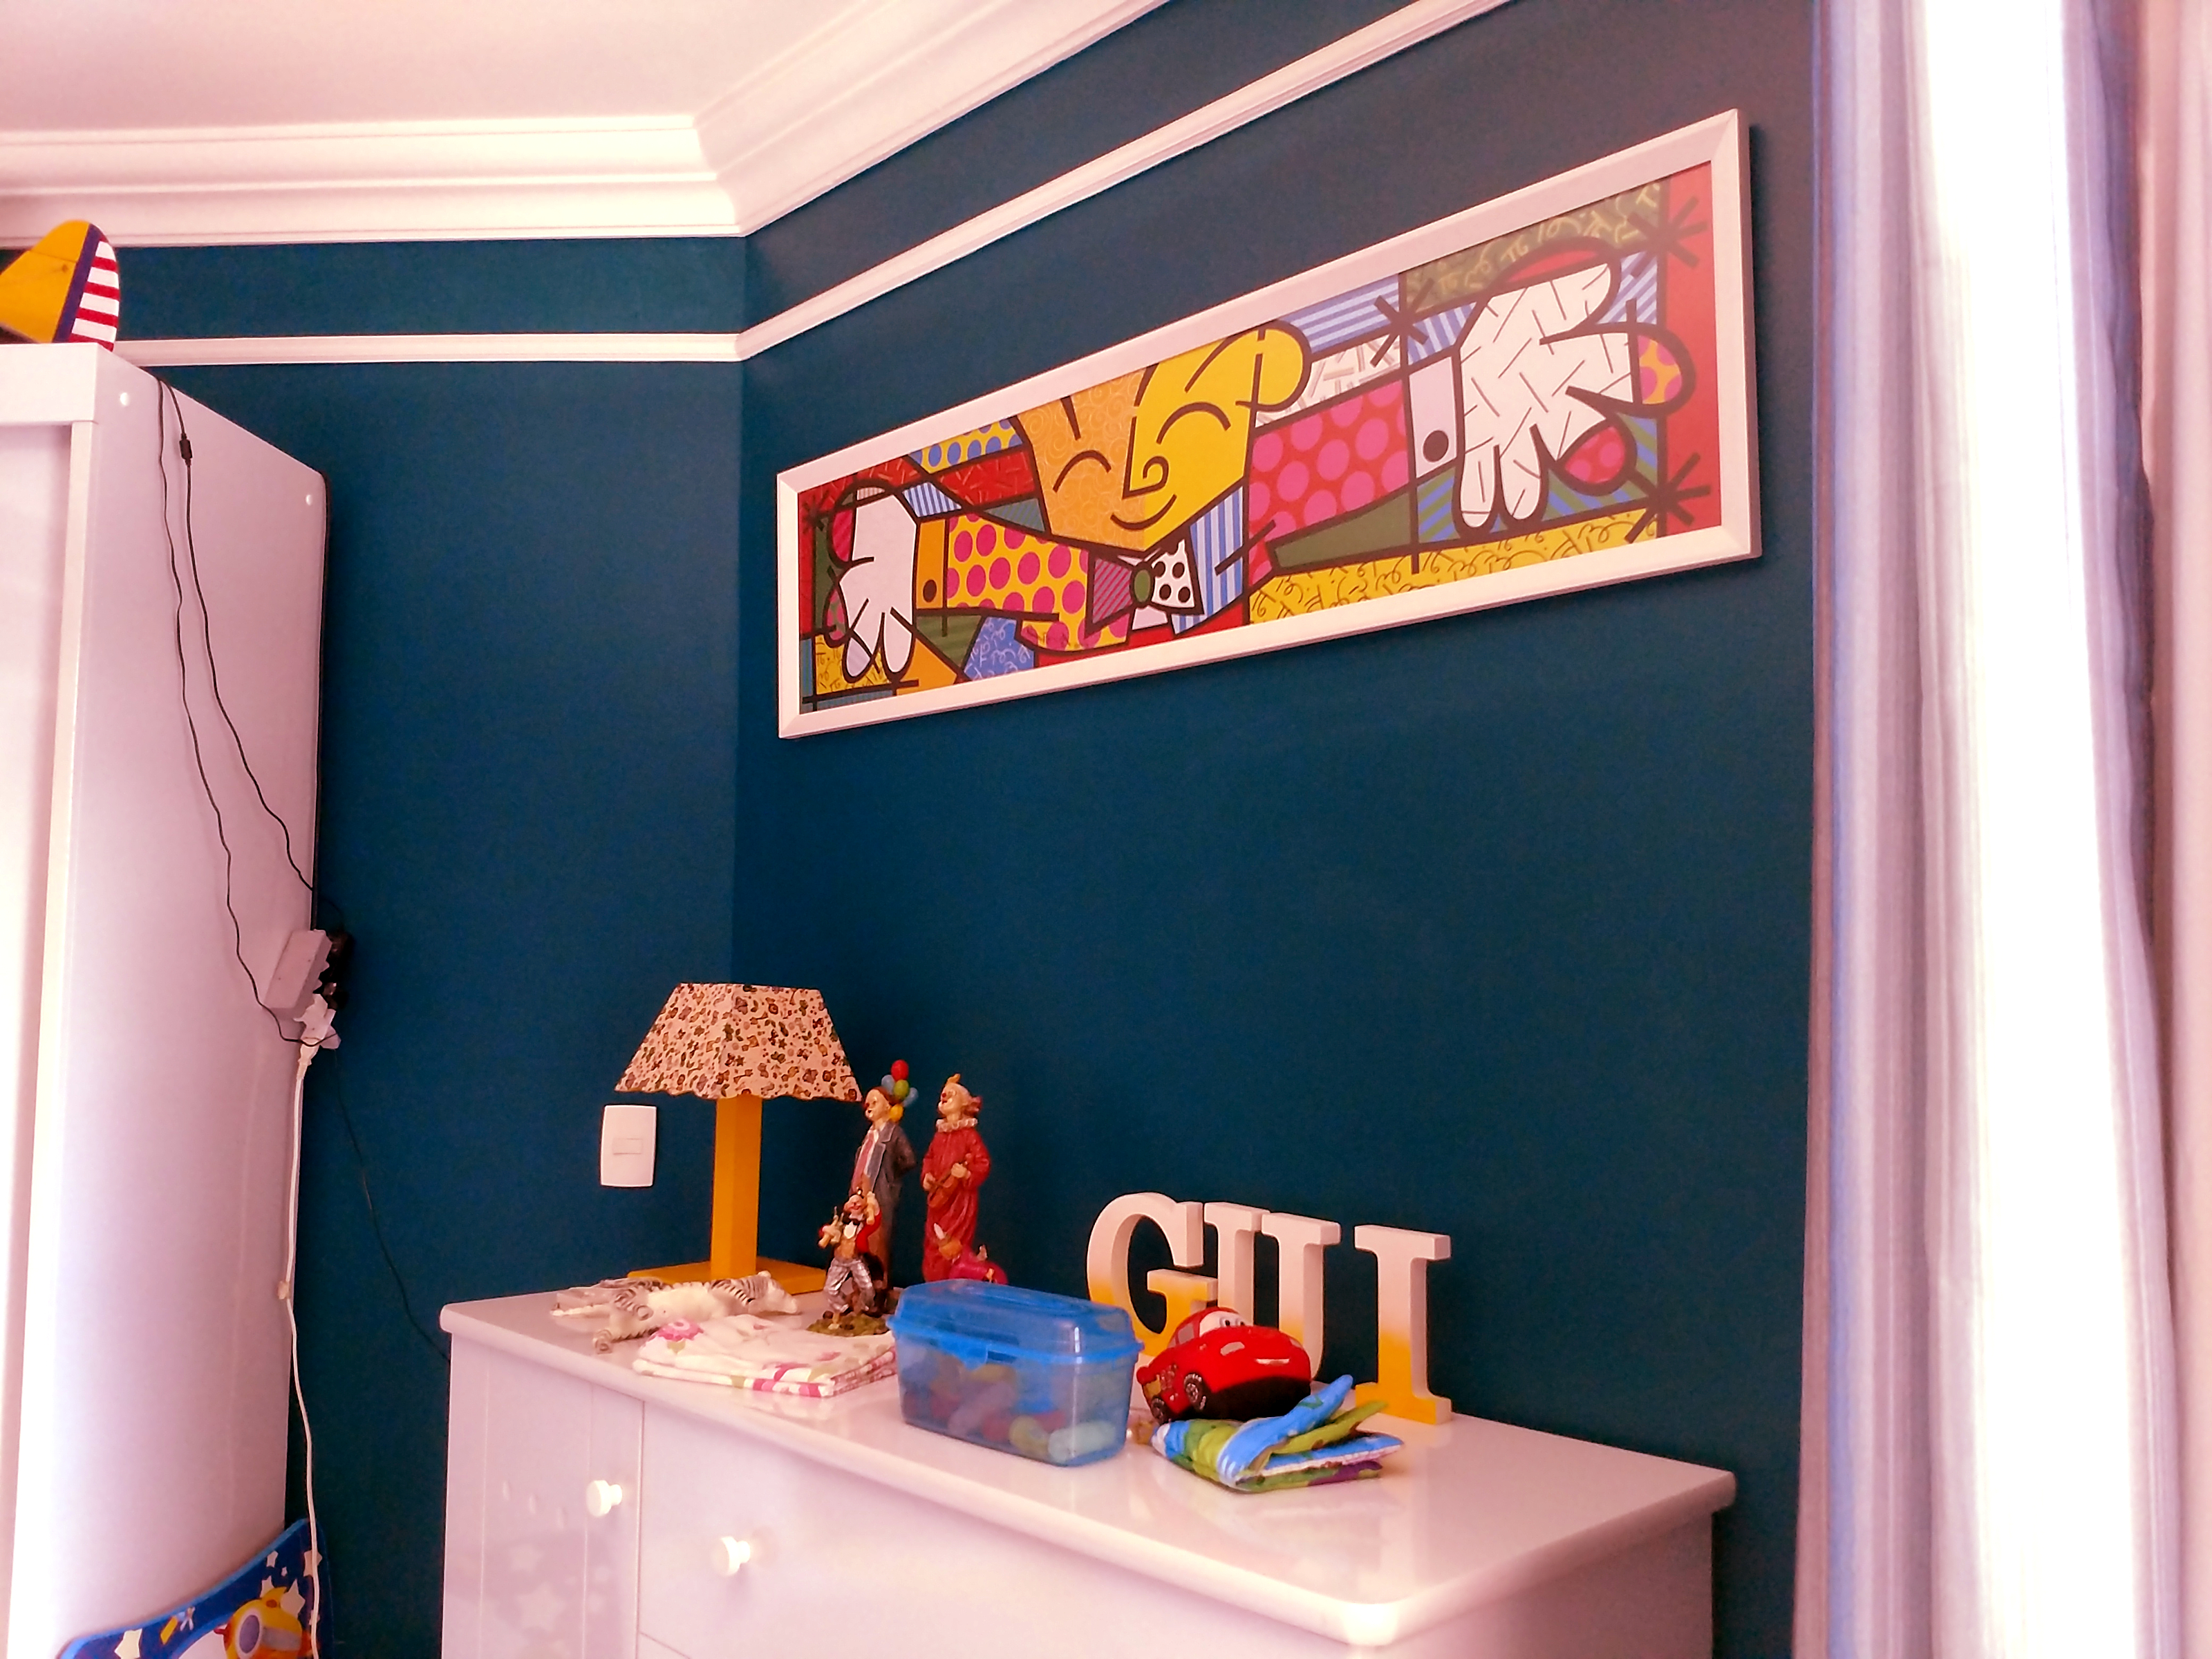
\includegraphics[width=5cm]{../data/img2.jpg}
    \includegraphics[width=5cm]{../code/imagem_2_melhorada.jpg}
    \caption{\emph{Esquerda:} Imagem 2 original. \emph{Direita:} Imagem 2 modificada.}
    \label{fig:result10}
\end{figure}

Foi possível concluir que na imagem de tamanho original não houve tanta diferença, pois os pontos X e Y não foram os mesmos utilizados para imagem patch, pois esses pontos foram perdidos e o algoritmo teve que ser executado novamente para a obtenção de um novo ponto, para poder aplicar na imagem 2. 

\newpage
\bibliographystyle{abntex2-alf}
\bibliography{references}

\end{document}
